\documentclass[a4paper, 11pt]{article}
\usepackage{wrapfig,blindtext} % For wraping text around image
\usepackage{comment} % enables the use of multi-line comments (\ifx \fi)
\usepackage{fullpage} % changes the margin
\usepackage{hyperref}
\usepackage{amsmath}
\usepackage{environ}
\usepackage{tabto,enumitem}
\usepackage{lipsum}
\usepackage{graphicx} % For image

\usepackage{tabto}
\usepackage{booktabs} % For formal tables

\usepackage[ruled]{algorithm2e} % For algorithms
\renewcommand{\algorithmcfname}{ALGORITHM}

\begin{document}

\noindent
\large\textbf{PROBLEM: 1} \hfill \textbf{Jemish Kishor Paghadar} \\
\normalsize\textbf{ SOEN-6011 (Software Engineering Processes)} \hfill \textbf{40080723} \\
{\centering\textbf{Function 4 :  $F(x)= \log_b x$} \\} 

\section{Description}
    In mathematics, the logarithm is the inverse function to exponentiation. That means the logarithm of a given number x is the exponent to which another fixed number, the base b, must be raised, to produce that number x. \\
    The exponential function that is $y=b^x$ has the inverse $x = b^y$. So, to express y as a function of x the logarithm was invented by John Napier in 1614.\cite{wiki}
    \newline
    \newline
    {\centering\textbf{$F(x)= \log_b x$}} is called "x is equal to b to the power y." This is equivalent to saying "y is the base-b logarithm of x."

\subsection{Domain \& Co-Domain}

    \begin{itemize}[noitemsep]
      \item The \textbf{domain} is the set of all \textbf{positive real numbers}.
      \item {$F(x)= \log_b x$} is not defined for negative values of x, or for 0. 
      \item It is defined for base \textbf{$b\neq1$ and $b>0$}. 
      \item The \textbf{co-domain} is the \textbf{set of all real numbers}. (Since the logarithmic function is the inverse of the exponential function, the domain of logarithmic function is the range of exponential function, and vice versa.). This function is continuous and one-to-one
    \end{itemize}


\section{Applications of logarithms}

    \begin{itemize}[noitemsep]
      \item It is used to simplify multiplication and division by converting these operations into addition and subtraction in \textbf{slide rule}. This is done by placing the numbers on a scale which is logarithmic. \cite{wiki}
      \item Logs are used in a variety of applications in sciences, some of the most common are: measuring loudness (decibels), measuring earthquake intensity (Richter scale), radioactive decay, and acidity ($pH= -\log_{10} [H^+]$). They are also essential in mathematics to solve certain exponential-type problems.
    \end{itemize}


\section{Properties of logarithms}
    \begin{minipage}{0.25\textwidth}
    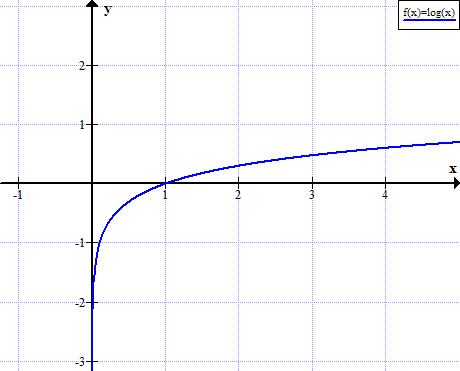
\includegraphics[width=\textwidth, height= 2.5 cm]{log_graph.png}
    \end{minipage}
    \begin{minipage}{0.9\textwidth}
    \begin{itemize}[noitemsep]
      \item The log of a product is the sum of the logs
      \item The sum of the logs is the log of the products
      \item The log of a quotient is the difference of the logs
      \item The difference of the logs is the log of the quotient
      \item The exponent on the argument is the coefficient of the log
      \item The coefficient of the log is the exponent on the argument
    \end{itemize}
    \end{minipage}

 
    
\begin{thebibliography}{9}
\bibitem{wiki}
\url{https://en.wikipedia.org/wiki/Logarithm}
\bibitem{rapidtables}
\url{https://www.rapidtables.com/math/algebra/Logarithm.html}
\end{thebibliography}

\end{document}
